\section{Collecte de Données}
\label{data_collection}

Dans notre projet de détection de détériorations de la route, la collecte de données est une étape fondamentale pour garantir la qualité et la fiabilité de notre modèle. Nous avons donc réalisé une nouvelle collecte de données en utilisant le robot, le module Arduino et notre application de collecte de données. Cette fois-ci, notre objectif était de collecter un maximum de données de différents types de détériorations de la route, afin d'en avoir suffisamment pour entraîner notre modèle d'apprentissage automatique.

Nous avons collecté environ quatre-vingt données (Figure \ref{data_collection_1}) de différentes détériorations de la route, notamment des dos d'âne, des failles, des fissures et des affaissements. Pour chaque type de détérioration, nous avons collecté en moyenne dix données par dégradation pour garantir la diversité de nos données.

Cependant, nous avons rencontré un problème avec notre carte arduino lors de la collecte de données. En effet, celle-ci n'a enregistré qu'une dizaine de données, sans que nous puissions identifier la cause de cette erreur. Bien que ce soit une déception, nous avons malgré tout pu collecter suffisamment de données avec l'application Android pour poursuivre notre projet de détection de détériorations de la route.

Dans l'ensemble, la collecte de données est une étape cruciale de notre projet, car la qualité des données collectées aura un impact direct sur la qualité et l'efficacité de notre modèle.

\begin{figure}
    \center
    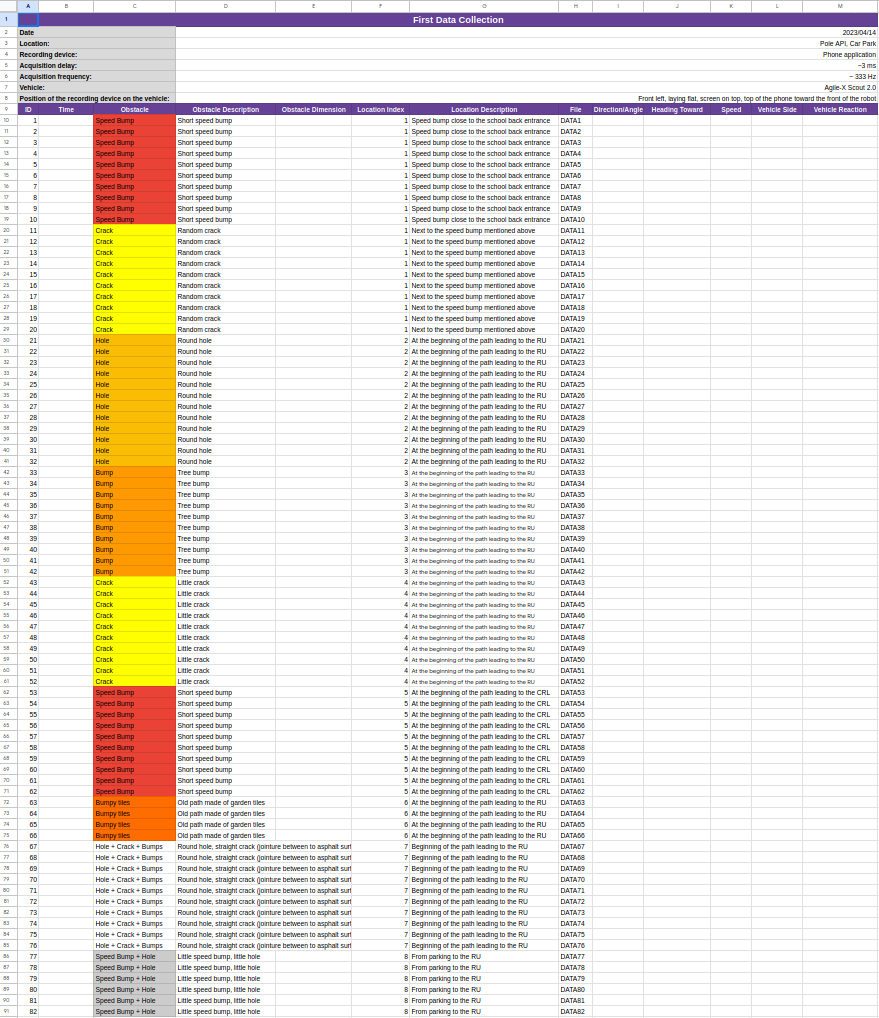
\includegraphics[scale=0.5]{img/data_collection_1.png}
    \caption{Tableur récapitulatif de la collecte de données}
    \label{data_collection_1}
\end{figure}